\documentclass[12pt]{article}
\usepackage[english]{babel}
\usepackage[utf8x]{inputenc}
\usepackage{amsmath}
\usepackage{tikz}
\usetikzlibrary{arrows,automata}
\begin{document}
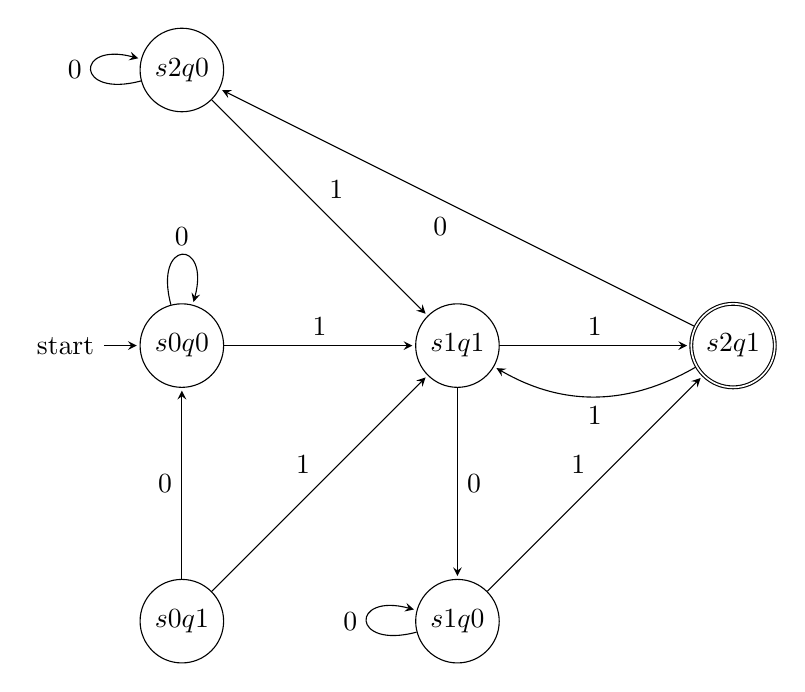
\begin{tikzpicture}[->,>=stealth,shorten >=1pt,auto,node distance=3.5cm,scale = 1,transform shape]
\node[state,initial] (s0q0) {$s0q0$};
\node[state] [below of=s0q0](s0q1) {$s0q1$};
\node[state] [right of=s0q1](s1q0) {$s1q0$};
\node[state] [right of=s0q0](s1q1) {$s1q1$};
\node[state] [above of=s0q0](s2q0) {$s2q0$};
\node[state,accepting] [right of=s1q1](s2q1) {$s2q1$};
\path (s0q0)	edge	[loop above]	node{$0$} (s0q0)
(s0q0)	edge		node{$1$} (s1q1)
(s0q1)	edge		node{$0$} (s0q0)
(s0q1)	edge		node{$1$} (s1q1)
(s1q0)	edge	[loop left]	node{$0$} (s1q0)
(s1q0)	edge		node{$1$} (s2q1)
(s1q1)	edge		node{$0$} (s1q0)
(s1q1)	edge		node{$1$} (s2q1)
(s2q0)	edge	[loop left]	node{$0$} (s2q0)
(s2q0)	edge		node{$1$} (s1q1)
(s2q1)	edge		node{$0$} (s2q0)
(s2q1)	edge	[bend left]	node{$1$} (s1q1)
;\end{tikzpicture}
\end{document}